\section{泛函的微分}
\label{sec:func-differential}

有限维中，一点处的梯度告诉我们目标沿每个方向的一阶变化。这就需要回答：对泛函，同样的事情怎样表述？方向上的变化率总可以先算，它能否合成一个线性近似，线性近似又能否写成一个梯度，这是三个不同的问题。

\subsection{方向微分与线性近似}
\label{sec:func-directional}

\paragraph{沿一条直线看}
给定候选$u$和扰动$\eta$，让实数$t$控制扰动的大小。整条曲线沿“方向”$\eta$移动，目标变成一元函数
\begin{equation}
 \phi(t)=J(u+t\eta).
 \label{eq:func-phi}
\end{equation}
这是最重要的一步化归：一元函数我们已经会求导。

下面用式~\eqref{eq:func-energy}的$E$计算一次。取$u(x)=x$，$\eta(x)=x(1-x)$，它们满足$\eta(0)=\eta(1)=0$，所以$x+t\eta$对每个$t$都可行。导数是$(x+t\eta)'=1+t(1-2x)$，代入后按$t$的幂次展开，需要三个积分：
\[
 \int_0^1(1-2x)\,\mathrm{d}x=0,\qquad
 \int_0^1(1-2x)^2\,\mathrm{d}x=\frac13,\qquad
 \int_0^1x\cdot x(1-x)\,\mathrm{d}x=\frac1{12}.
\]
再加上$\int_0^1x^2(1-x)^2\,\mathrm{d}x=\frac1{30}$和$E(x)=\frac23$，得到
\begin{equation}
 \phi(t)=\frac23+\frac{t}{12}+\frac{11}{60}t^2.
 \label{eq:func-phi-example}
\end{equation}
所以$\phi'(0)=1/12$。图~\ref{fig:func-direction-family}的(a)是这一族曲线，(b)是$\phi$及其切线。注意这里求导的变量是$t$，不是$x$：$u'(x)$描述一条固定曲线的陡峭程度，$\phi'(0)$描述整条曲线改动时目标的响应。

\begin{BookInlineFigure}
  \centering
  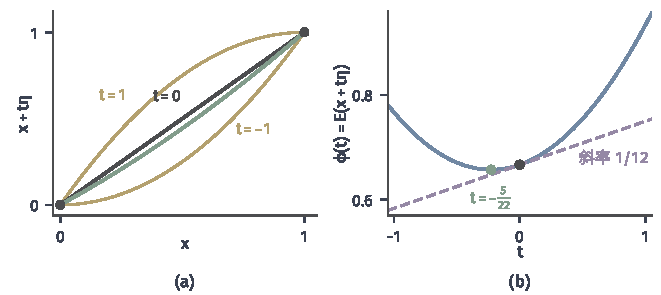
\includegraphics[width=112mm]{figures/05-optimization/08-functional-optimization/matplotlib/func-direction-family/figure.pdf}
  \caption{沿一个方向改动整条曲线。(a)$u=x$（深灰）和$\eta=x(1-x)$给出的曲线族$x+t\eta$，黄色$t=\pm1$，绿色$t=-5/22$，端点不动。(b)$\phi(t)=E(x+t\eta)$，紫色虚线是$t=0$处的切线，斜率$1/12$；绿点是这条直线上的最小点$t=-5/22$。}
  \label{fig:func-direction-family}
\end{BookInlineFigure}

$\phi$在$t=-5/22$处最小，说明沿这个方向还能下降，$x$不是极小点。这个判断只用了一元微积分。

\begin{definition}[方向导数]
\label{def:func-directional}
设$X$是实赋范空间，$J(u)$有限，$\eta\in X$，且$t>0$充分小时$J(u+t\eta)$有限。若极限
\begin{equation}
 J'(u;\eta)=\lim_{t\downarrow0}\frac{J(u+t\eta)-J(u)}{t}
 \label{eq:func-directional}
\end{equation}
存在且有限，称它为$J$在$u$处沿$\eta$的\term{方向导数}（directional derivative）。
\end{definition}

定义只取$t\downarrow0$的单侧极限，因为有约束时常常只能朝一侧走。方向导数只回答一条直线上的问题，把所有方向的答案放在一起，未必是线性函数。在$L^2(0,1)$上取$J(u)=\int_0^1\lvert u\rvert\,\mathrm{d}x$，由齐次性直接得到$J'(0;\eta)=\int_0^1\lvert\eta\rvert\,\mathrm{d}x$。它对$\eta$不可加，$J'(0;\eta)+J'(0;-\eta)$也不为零。这与$\lvert x\rvert$在原点的尖角相同。

\paragraph{线性且连续：Gâteaux微分}
有限维中，光滑函数的方向导数是$\nabla f(\bm{x})^\top\bm{d}$，对$\bm{d}$线性。线性是我们想要的结构，无限维中还要多要求一件事：连续。有限维的线性函数自动连续，无限维的线性泛函不然。

\begin{definition}[Gâteaux微分]
\label{def:func-gateaux}
若$J'(u;\eta)$对每个$\eta\in X$存在，且$\eta\mapsto J'(u;\eta)$是$X$上的连续线性泛函，称$J$在$u$处\term{Gâteaux可微}（Gâteaux differentiable），称这个泛函为$J$在$u$处的\term{Gâteaux微分}（Gâteaux derivative），记作$DJ(u)\in X^*$，即
\begin{equation}
 DJ(u)[\eta]=J'(u;\eta).
 \label{eq:func-gateaux}
\end{equation}
\end{definition}

线性中已经包含$J'(u;-\eta)=-J'(u;\eta)$，所以这时$t\to0$的双侧极限也存在。Gâteaux微分还是逐方向定义的：对每个固定的$\eta$，$t$足够小时余项才小，“足够小”的程度可以随方向变化。

\paragraph{一致的余项：Fréchet微分}
真正的线性近似要求：只要扰动在范数下小，余项就比范数小，不管扰动沿哪个方向。

\begin{definition}[Fréchet微分]
\label{def:func-frechet}
设$J$在$u$的某邻域内有限。若存在$\xi\in X^*$使
\begin{equation}
 \lim_{\lVert\eta\rVert\to0}\frac{\lvert J(u+\eta)-J(u)-\xi(\eta)\rvert}{\lVert\eta\rVert}=0,
 \label{eq:func-frechet}
\end{equation}
称$J$在$u$处\term{Fréchet可微}（Fréchet differentiable），$\xi$称为Fréchet微分。
\end{definition}

两个定义的差别只在极限的取法。Gâteaux微分固定形状，只缩小幅度；Fréchet微分允许形状和幅度同时变化。无限维中形状可以无穷多，这个差别才变得实质。

\paragraph{一个Gâteaux可微而非Fréchet可微的泛函}
下面的例子说明，这个差别由范数决定。考虑
\begin{equation}
 S(u)=\int_0^1\sin\bigl(u(x)\bigr)\,\mathrm{d}x.
 \label{eq:func-sin}
\end{equation}
先在$X=L^1(0,1)$的$u=0$处计算方向导数。差商的被积函数$\sin(t\eta)/t$逐点趋于$\eta$，并被可积函数$\lvert\eta\rvert$控制，由控制收敛定理，
\[
 S'(0;\eta)=\int_0^1\eta(x)\,\mathrm{d}x.
\]
它线性，并且不超过$\lVert\eta\rVert_1$，所以$S$在$0$处Gâteaux可微。

再测试余项。取图~\ref{fig:func-spike-frechet}(a)的尖峰$\eta_k=\pi\mathbf{1}_{[0,1/k]}$，幅度始终是$\pi$，宽度趋于零。余项为
\[
 S(\eta_k)-S(0)-\int_0^1\eta_k\,\mathrm{d}x=\frac1k\bigl(\sin\pi-\pi\bigr)=-\frac{\pi}{k}.
\]
而$\lVert\eta_k\rVert_1=\pi/k$，比值的绝对值恒等于$1$，不趋于零。所以$S$在$L^1$中不是Fréchet可微的。

\begin{BookInlineFigure}
  \centering
  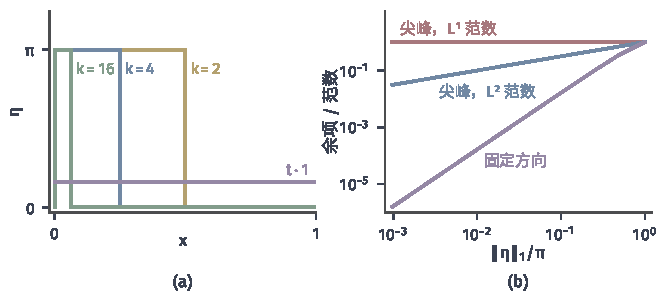
\includegraphics[width=112mm]{figures/05-optimization/08-functional-optimization/matplotlib/func-spike-frechet/figure.pdf}
  \caption{同一泛函$S(u)=\int_0^1\sin u\,\mathrm{d}x$在$u=0$处的余项。(a)尖峰扰动$\pi\mathbf{1}_{[0,1/k]}$（$k=2,4,16$）与固定方向的缩小$t\cdot1$（紫色）。(b)余项除以范数：尖峰在$L^1$范数下恒为$1$（红），在$L^2$范数下按$k^{-1/2}$衰减（蓝）；固定方向$t\cdot1$按$t^2$衰减（紫）。}
  \label{fig:func-spike-frechet}
\end{BookInlineFigure}

换成$X=L^2(0,1)$，同一个尖峰的范数是$\lVert\eta_k\rVert_2=\pi k^{-1/2}$，比$L^1$范数大得多，比值变成$k^{-1/2}\to0$。这不是巧合。由Taylor公式，逐点有
\[
 \lvert\sin(u+\eta)-\sin u-\eta\cos u\rvert\leq\frac12\eta^2.
\]
两边积分，得到
\[
 \Bigl\lvert S(u+\eta)-S(u)-\int_0^1\eta\cos u\,\mathrm{d}x\Bigr\rvert\leq\frac12\lVert\eta\rVert_2^2.
\]
所以$S$在$L^2$中处处Fréchet可微。在$L^1$中，窄而高的尖峰范数很小，函数值的改动却不小；$L^2$范数对尖峰更敏感，把它们排除在“小扰动”之外。讨论可微性时必须说清范数。

\paragraph{两种微分的关系}
下面的定理说明，Fréchet可微更强，以及在什么条件下两者相同。

\begin{theorem}[Gâteaux与Fréchet]
\label{thm:func-gateaux-frechet}
设$J$在$u$的某邻域内有限。
\begin{enumerate}
 \item 若$J$在$u$处Fréchet可微，则$J$在$u$处Gâteaux可微，且$DJ(u)=\xi$。
 \item 若$J$在$u$的邻域内Gâteaux可微，且映射$v\mapsto DJ(v)$在$u$处从$X$到$X^*$连续，则$J$在$u$处Fréchet可微。
\end{enumerate}
\end{theorem}

\begin{proof}
(1)固定$\eta\neq0$，在式~\eqref{eq:func-frechet}中用$t\eta$代替$\eta$，$t\downarrow0$时$\lVert t\eta\rVert\to0$。两边除以$t$，得到差商趋于$\xi(\eta)$。

(2)取$\lVert\eta\rVert$足够小，使线段$u+t\eta$（$t\in[0,1]$）落在邻域内。$\phi(t)=J(u+t\eta)$在$[0,1]$上可导，$\phi'(t)=DJ(u+t\eta)[\eta]$。由Lagrange中值定理，存在$\theta\in(0,1)$，使
\[
 J(u+\eta)-J(u)=DJ(u+\theta\eta)[\eta].
\]
两边减去$DJ(u)[\eta]$，再用对偶范数的定义，得到
\[
 \bigl\lvert J(u+\eta)-J(u)-DJ(u)[\eta]\bigr\rvert\leq\lVert DJ(u+\theta\eta)-DJ(u)\rVert\,\lVert\eta\rVert.
\]
由连续性，$\lVert\eta\rVert\to0$时右端的第一个因子趋于零。
\end{proof}

这解释了$S$在$L^1$中的情形：$DS(v)$是乘以$\cos v$的积分，$L^1$范数很小的尖峰可以让$\cos v$在一小段上改变一个固定的量，所以微分在$X^*=L^\infty$中不连续，第二条的条件不满足。

三个层次可以列表比较。

\begin{BookInlineTable}
  \centering
  \caption{一阶信息的三个层次。}
  \label{tab:func-derivative-levels}
  \begin{tabular}{lll}
    \toprule
    层次 & 要求 & 不满足下一层的例子\\
    \midrule
    方向导数 & 每条直线上有导数 & $\int_0^1\lvert u\rvert\,\mathrm{d}x$ 在 $u=0$\\
    Gâteaux微分 & 上述导数线性连续 & $\int_0^1\sin u\,\mathrm{d}x$ 在 $L^1$\\
    Fréchet微分 & 余项对方向一致 & ---\\
    \bottomrule
  \end{tabular}
\end{BookInlineTable}

\paragraph{能量的展开}
回到$E$。对$u,\eta\in H^1(0,1)$，把平方展开，不做任何近似：
\begin{equation}
 E(u+\eta)=E(u)+\int_0^1\bigl(u'\eta'+u\eta\bigr)\,\mathrm{d}x+\frac12\lVert\eta\rVert_{H^1}^2.
 \label{eq:func-energy-expansion}
\end{equation}
中间一项是$\eta$的线性泛函。由Cauchy--Schwarz不等式，它的绝对值不超过$\lVert u\rVert_{H^1}\lVert\eta\rVert_{H^1}$，所以连续。余项是$\frac12\lVert\eta\rVert_{H^1}^2$，比$\lVert\eta\rVert_{H^1}$高一阶。因此$E$在$H^1$中处处Fréchet可微，
\begin{equation}
 DE(u)[\eta]=\int_0^1\bigl(u'\eta'+u\eta\bigr)\,\mathrm{d}x.
 \label{eq:func-energy-derivative}
\end{equation}
取$u=x$，$\eta=x(1-x)$，右端是$\int_0^1(1-2x)\,\mathrm{d}x+\frac1{12}=\frac1{12}$，与式~\eqref{eq:func-phi-example}一致。长度目标也可以同样处理：$G(p)=\sqrt{1+p^2}$满足$0<G''\leq1$，由Taylor公式，余项不超过$\frac12\lVert\eta'\rVert_2^2$，所以$\ell$在$H^1$中Fréchet可微。

\subsection{Hilbert梯度}
\label{sec:func-hilbert-gradient}

微分$DJ(u)$是一个把方向读成数的线性泛函，它是“行向量”。梯度下降需要的却是一个能和候选相加的“列向量”。本小节要回答的问题是：怎样把微分转成梯度？答案取决于内积。

\paragraph{有限维中内积就已经起作用}
把向量和方向配对的是微分$Df(\bm{x})[\bm{d}]=\nabla f(\bm{x})^\top\bm{d}$，这里的$\nabla f$其实默认了欧氏内积。换一个内积，由对称正定矩阵$\bm{M}$给出：
\[
 \langle\bm{x},\bm{y}\rangle_{\bm{M}}=\bm{x}^\top\bm{M}\bm{y}.
\]
这时梯度应当是满足下式的向量$\bm{g}$，内积下读出的就是同一个微分：
\[
 \bm{g}^\top\bm{M}\bm{d}=\nabla f(\bm{x})^\top\bm{d}\qquad\text{对每个}\ \bm{d}.
\]
解出来就是
\begin{equation}
 \bm{g}=\bm{M}^{-1}\nabla f(\bm{x}).
 \label{eq:func-metric-gradient}
\end{equation}

用第~\ref{chap:smooth-foundations}章的例子$f(\bm{x})=\frac12(x_1^2+9x_2^2)$看，在$\bm{x}=(9,1)$处，$\nabla f=(9,9)$。取$\bm{M}=\operatorname{diag}(1,9)$，它是这个目标的Hessian，代入式~\eqref{eq:func-metric-gradient}，
\[
 \bm{g}=(9,1).
\]
图~\ref{fig:func-metric-gradient}中，黄色箭头是欧氏梯度方向的一步，绿色箭头沿$-\bm{g}$，一步直达原点。同一个微分，在两个内积下给出两个不同的梯度。“最速下降方向”依赖怎样度量步长的长度。

\begin{BookInlineFigure}
  \centering
  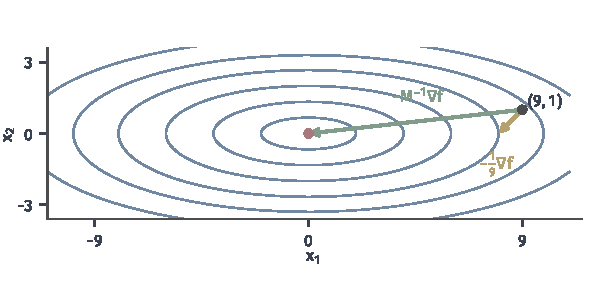
\includegraphics[width=100mm]{figures/05-optimization/08-functional-optimization/matplotlib/func-metric-gradient/figure.pdf}
  \caption{同一个微分在两个内积下的梯度。蓝色为$f=\frac12(x_1^2+9x_2^2)$的等高线，出发点$(9,1)$。黄色箭头是步长$1/9$的欧氏负梯度步，绿色箭头是$\bm{M}=\operatorname{diag}(1,9)$内积下步长$1$的负梯度步，终点是最优解（红点）。}
  \label{fig:func-metric-gradient}
\end{BookInlineFigure}

\paragraph{函数空间中的梯度}
有限维中$\bm{M}$可逆，这个转换永远可以做。在Hilbert空间中，转换由Riesz表示定理完成：$H$上的每个连续线性泛函$\xi$，都存在唯一的$w\in H$，使$\xi(\eta)=\langle w,\eta\rangle_H$对所有$\eta\in H$成立。

\begin{definition}[Hilbert梯度]
\label{def:func-hilbert-gradient}
设$H$是实Hilbert空间，$J$在$u$处沿$H$的方向Gâteaux可微。称满足
\begin{equation}
 DJ(u)[\eta]=\bigl\langle\nabla_HJ(u),\eta\bigr\rangle_H\qquad(\eta\in H)
 \label{eq:func-hilbert-gradient}
\end{equation}
的唯一元素$\nabla_HJ(u)\in H$为$J$在$u$处的\term{Hilbert梯度}（Hilbert gradient）。
\end{definition}

由Cauchy--Schwarz不等式，在$\lVert\eta\rVert_H=1$的方向中，$DJ(u)[\eta]$在$\eta$平行于$\nabla_HJ(u)$时最大，所以它确实是“上升最快的方向”，只是这里的“单位长度”用$H$的范数计量。

\paragraph{同一个微分的三个梯度}
下面算一个具体例子。对$E$在$u=x$处，方向取$\bm{V}=H^1_0(0,1)$。由式~\eqref{eq:func-energy-derivative}和$\int_0^1\eta'\,\mathrm{d}x=\eta(1)-\eta(0)=0$，得到
\begin{equation}
 DE(x)[\eta]=\int_0^1x\,\eta(x)\,\mathrm{d}x.
 \label{eq:func-de-at-x}
\end{equation}
这一个线性泛函，用三种内积表示。

第一种是$L^2$内积。式~\eqref{eq:func-de-at-x}已经写成了$\langle x,\eta\rangle_2$，所以$L^2$梯度是
\[
 w_1(x)=x.
\]
第二种内积只用导数：
\[
 \langle v,\eta\rangle_{\bm{V}}=\int_0^1v'\eta'\,\mathrm{d}x.
\]
由Poincaré不等式它是$\bm{V}$上的内积，$\bm{V}$在其下完备。要找$w_2\in\bm{V}$，使它在这个内积下读出式~\eqref{eq:func-de-at-x}。分部积分，边界项因$\eta$在端点为零而消失，问题化成$-w_2''=x$，$w_2(0)=w_2(1)=0$。解得
\[
 w_2(x)=\frac{x-x^3}{6}.
\]
第三种是$H^1$内积$\int_0^1(v'\eta'+v\eta)\,\mathrm{d}x$。同样分部积分，问题化成$-w_3''+w_3=x$，$w_3(0)=w_3(1)=0$。解得
\[
 w_3(x)=x-\frac{\sinh x}{\sinh1}.
\]

三个函数画在图~\ref{fig:func-three-gradients}中，形状和大小都不同，但它们表示同一个微分。用$\eta=x(1-x)$检验，三种内积给出的都是$1/12$。例如第二种：
\[
 \int_0^1\frac{1-3x^2}{6}(1-2x)\,\mathrm{d}x=\frac1{12}.
\]

\begin{BookInlineFigure}
  \centering
  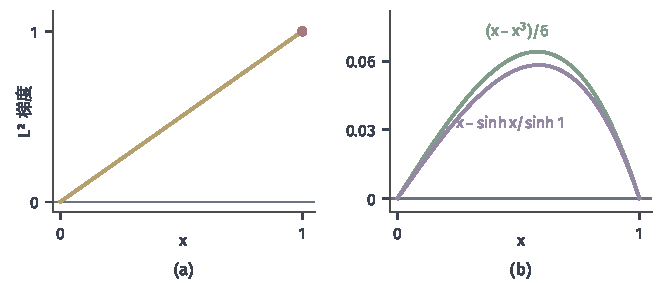
\includegraphics[width=112mm]{figures/05-optimization/08-functional-optimization/matplotlib/func-three-gradients/figure.pdf}
  \caption{$E$在$u=x$处同一微分的三个梯度。(a)$L^2$梯度$w_1=x$，在$x=1$处不为零（红点），不是允许的扰动方向。(b)绿色$w_2$对应内积$\int v'\eta'$，紫色$w_3$对应$H^1$内积，二者都在端点为零。注意两幅图的纵轴尺度相差十倍以上。}
  \label{fig:func-three-gradients}
\end{BookInlineFigure}

它们的差别有实际后果。$w_1$在$x=1$处等于$1$，沿它走一步会破坏端点条件，它不是$\bm{V}$中的元素：$\bm{V}$在$L^2$内积下不完备，Riesz定理在这里并没有保证梯度落在$\bm{V}$内。$w_2,w_3$是$\bm{V}$中的元素，沿它们走仍然可行。

$w_3$还有一个特别之处。$E$的二次项正是$H^1$内积，这和上面的$\bm{M}$取Hessian相同，所以$u-w_3=\sinh x/\sinh1$一步到位。这条曲线就是图~\ref{fig:func-feasible-directions}中绿色的候选，它的能量约为$0.6565$，比$E(x)=2/3$低；第~\ref{sec:func-integral}节将确认它就是极小点。

\paragraph{函数梯度与坐标梯度}
把函数离散成结点向量，函数的梯度与向量的梯度是什么关系？看最简单的$J(u)=\frac12\int_0^1u^2\,\mathrm{d}x$，它的$L^2$梯度是$u$。离散成$J_n(\bm{u})=\frac{\Delta}{2}\sum_iu_i^2$，向量梯度的分量是$\Delta u_i$，随网格加密趋于零。

要得到函数的梯度，必须除以$\Delta$。这正是式~\eqref{eq:func-metric-gradient}中取$\bm{M}=\Delta\bm{I}$，也就是离散$L^2$内积$\Delta\sum_iu_iv_i$。向量梯度依赖离散的细节，函数梯度依赖选定的内积，从前者到后者要乘以内积矩阵的逆。

\paragraph{梯度可以不存在}
有限维中，每个线性函数都连续，所以任何内积下都有梯度。无限维不是这样。考虑$E_0(u)=\frac12\int_0^1u'^2\,\mathrm{d}x$，在$\bm{V}=H^1_0(0,1)$的帐篷函数$u=\min\{x,1-x\}$处，把积分在$x=\frac12$处分开：
\[
 DE_0(u)[\eta]=\int_0^{1/2}\eta'\,\mathrm{d}x-\int_{1/2}^1\eta'\,\mathrm{d}x=2\,\eta\bigl(\tfrac12\bigr).
\]
微分只读取中点的值。在内积$\int v'\eta'$下，由定义，$\nabla E_0(u)=u$，这是图~\ref{fig:func-tent-gradient}(a)的帐篷。

在$L^2$内积下，$\eta\mapsto2\eta(\frac12)$不连续。取中点处高度为$1$、半宽为$1/k$的小帐篷$\eta_k$，有
\[
 DE_0(u)[\eta_k]=2,\qquad\lVert\eta_k\rVert_2^2=\frac{2}{3k}\to0.
\]
没有$L^2$函数能表示这个读取，$L^2$梯度不存在。形式上的“梯度”$-u''$是中点处质量为$2$的点质量，它不是函数。

把问题离散，就能看到这一点。线性元的结点向量梯度只在中点非零，等于$2$；转成离散$L^2$梯度要除以$\Delta=1/n$，于是高度为$2n$。图~\ref{fig:func-tent-gradient}(b)的尖峰随网格加密无限增高，没有极限函数。

\begin{BookInlineFigure}
  \centering
  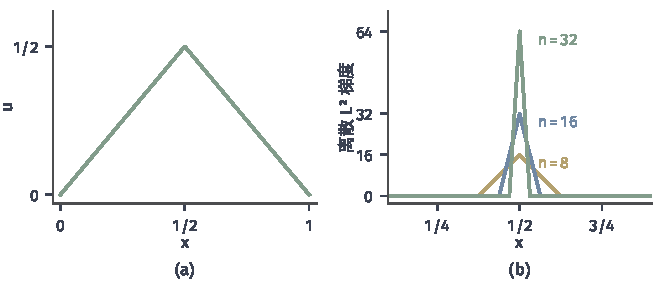
\includegraphics[width=112mm]{figures/05-optimization/08-functional-optimization/matplotlib/func-tent-gradient/figure.pdf}
  \caption{帐篷函数$u=\min\{x,1-x\}$在$E_0=\frac12\int u'^2\,\mathrm{d}x$下的梯度。(a)在内积$\int v'\eta'$下，梯度就是$u$本身。(b)离散$L^2$梯度，在$n=8,16,32$段网格上中点高度为$2n$，网格越细越高，没有极限函数。}
  \label{fig:func-tent-gradient}
\end{BookInlineFigure}

\paragraph{选错内积的代价}
即使$L^2$梯度存在，用它做下降也有问题。对式~\eqref{eq:func-energy}用$n$段线性元离散，在两种内积下跑步长为$1/L$的梯度下降，$L$是对应内积下的光滑常数。

$L^2$内积下，$L$约等于离散二阶差分的最大特征值$4n^2$。$n=16,32,64$时步长分别约为$9.9\times10^{-4}$、$2.4\times10^{-4}$、$6.1\times10^{-5}$，网格每加密一倍，步长缩小到四分之一。原因是$-u''$是无界的运算，函数摆动越快，它放大得越多。

内积$\int v'\eta'$下，相应的算子把频率$k$的分量放大$1+(k\pi)^{-2}$倍，$L\approx1.10$与网格无关。图~\ref{fig:func-gd-metric}显示了结果，绿线几步就到达机器精度，黄线$100$步后目标差仍在$10^{-3}$到$10^{-2}$之间，而且网格越细越慢。

\begin{BookInlineFigure}
  \centering
  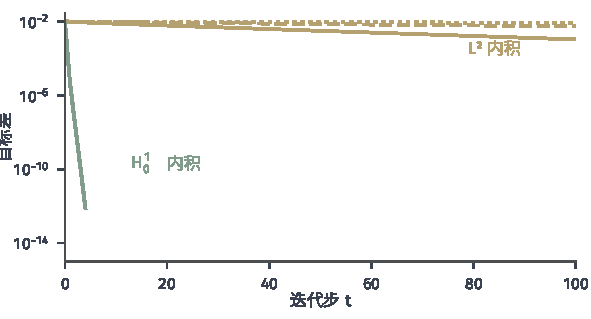
\includegraphics[width=100mm]{figures/05-optimization/08-functional-optimization/matplotlib/func-gd-metric/figure.pdf}
  \caption{线性元离散的$E$上，步长$1/L$的梯度下降从$u=x$出发的目标差。黄色为$L^2$内积，绿色为内积$\int v'\eta'$；实线、虚线、点线分别是$n=16,32,64$。绿色三条线重合，收敛不随网格变慢。}
  \label{fig:func-gd-metric}
\end{BookInlineFigure}

这和第~\ref{chap:second-order-methods}章讲的二阶信息是同一件事：选一个接近Hessian的内积，就是做预条件。函数空间的视角补充的是：网格加密时，好的内积让迭代次数保持不变，这件事在单个有限维问题里看不出来。

\paragraph{类比到哪里为止}
下面把向量与函数的对应关系补完，并列出类比失效的地方。

\begin{BookInlineTable}
  \centering
  \caption{一阶信息的对应与差别。}
  \label{tab:func-gradient-analogy}
  \begin{tabular}{lll}
    \toprule
    & 有限维 & 函数空间\\
    \midrule
    闭球 & 紧 & 不紧，只有弱序列紧\\
    范数 & 彼此等价 & 不等价，决定可微性\\
    线性泛函 & 自动连续 & 可以不连续\\
    梯度 & 任何内积下都存在 & 可能不存在\\
    Hessian & 有界 & 在 $L^2$ 中可以无界\\
    \bottomrule
  \end{tabular}
\end{BookInlineTable}

可以这样记：有限维的直觉在选定空间之后才能使用，选空间这一步是函数问题特有的。
